\documentclass[border=4pt]{standalone}
\usepackage{amsmath,amssymb}
\usepackage{tikz}
\begin{document}
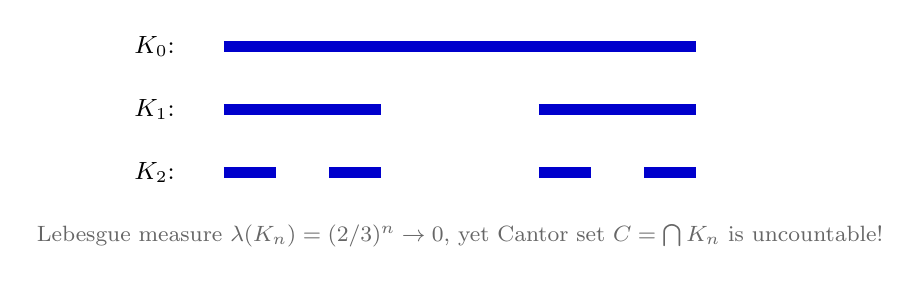
\begin{tikzpicture}[font=\small]
  % K_0
  \node[left] at (0, 2.4) {$K_0$:};
  \draw[line width=4pt, blue!80!black] (0.5, 2.4) -- (6.5, 2.4);

  % K_1
  \node[left] at (0, 1.6) {$K_1$:};
  \draw[line width=4pt, blue!80!black] (0.5, 1.6) -- (2.5, 1.6);
  \draw[line width=4pt, blue!80!black] (4.5, 1.6) -- (6.5, 1.6);

  % K_2
  \node[left] at (0, 0.8) {$K_2$:};
  \draw[line width=4pt, blue!80!black] (0.5, 0.8) -- (1.16, 0.8);
  \draw[line width=4pt, blue!80!black] (1.84, 0.8) -- (2.5, 0.8);
  \draw[line width=4pt, blue!80!black] (4.5, 0.8) -- (5.16, 0.8);
  \draw[line width=4pt, blue!80!black] (5.84, 0.8) -- (6.5, 0.8);

  % Labels
  \node[font=\footnotesize, text=gray!80!black] at (3.5, 0.0) 
    {Lebesgue measure $\lambda(K_n) = (2/3)^n \to 0$, yet Cantor set $C = \bigcap K_n$ is uncountable!};
\end{tikzpicture}
\end{document}